\documentclass[twocolumn]{article}

% \usepackage{../needed}
\usepackage{xcolor}
\usepackage{wrapfig}
\usepackage{empheq}
\usepackage{amsmath}
\usepackage[a4paper, margin=0.95in]{geometry}

\definecolor{c3}{RGB}{80, 90, 140}
\definecolor{c2}{RGB}{230, 240, 255}

\newcommand{\coloredeq}[2]{\begin{empheq}[box=\colorbox{c2}]{align}\label{#1}#2\end{empheq}}


\title{PHYS213 Paper}
\author{Alfaifi, Ammar}
\date{\today}

\begin{document}
    \maketitle
    \begin{abstract}
        Up to now, we only considered, in prevoius chapters, the quantum mechanics in one dimensional
        space. We need to extend the quantumn idea in more degree of freedom, i.e., for 3D space, as well
        as the centeral force for atoms. Further, we aim to distinguish the \emph{sharp} observables.
    \end{abstract}
    \section{\color{c3}\MakeUppercase{Particle in a Three-Dimensional Box}}
        \paragraph{} % (fold)
        \label{par:Particle in A Three-Dimensional Box}
        We consider a Cubic box whose length $L$. Inside this box a free particle collide
        with \emph{smooth} elastically with box' walls, presrving the magnitude of each
        momentum component, in addition to the total energy. This means that the particle occupies the 
        the region $0<x, y, z<L$.
        % paragraph Particle in A Three-Dimensional Box (end)

        \paragraph{}
        Since this is a three dimensional coordinate, the wavefunction $\Psi$ is a function of
        the position vector $\vec{r}=(x, y, z)$. The probability density
        $|\Psi(\vec{r})|^2$ is a \emph{probability per volume}. Thus, the \textbf{Schr\"odinger's
        equation} is given by \coloredeq{3D box equation}{
            -\frac{\hbar}{2m} \nabla^2\Psi + U(\vec{r}) = i\hbar \frac{\partial \Psi}{\partial t}
        }

    \section{\color{c3}\MakeUppercase{centeral forces and angular momentum}}
        \paragraph{}
        \begin{wrapfigure}{r}{0.5\linewidth}
            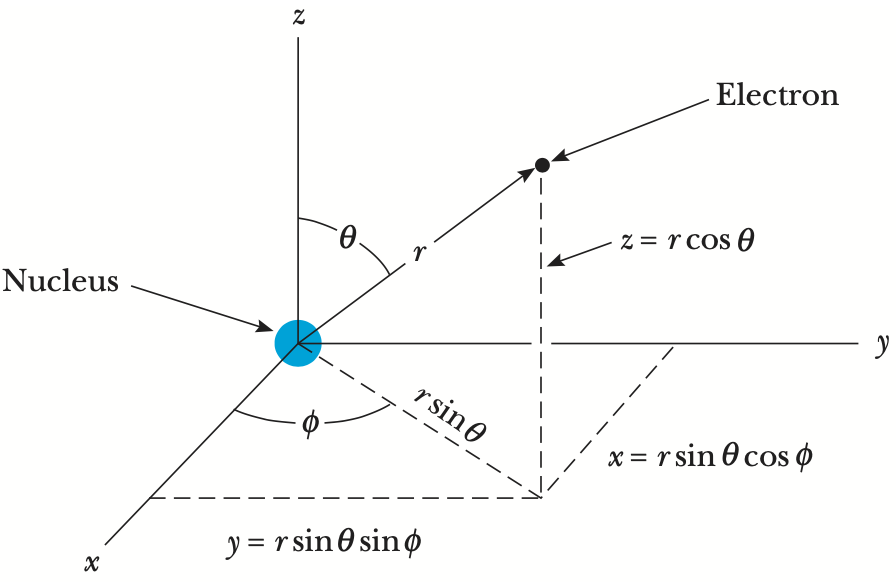
\includegraphics[width=0.9\linewidth]{figures/spherical-coordinates}
            \caption{Spherical coordinates for an electron.}
            \label{fig:spherical coordinates}
        \end{wrapfigure}

        In contrast of the Cartesain coordinates, we turn our attention to the spherical coordinates,
        since it is more convenient while dealing with \textbf{centeral forces}. In atoms situation,
        the centeral force is the Columb attractive force originating from the nucleus, affecting on
        electrons. Now the vector position becomes $\vec{r} = (r, \theta, \phi)$, as in Figure~\ref{fig:spherical coordinates}. It is important to
        note that in orbiting electron, its angular momentum $\vec{L}$ is only \emph{shart} along 
        a chosen axis while the others components being "fuzzy". Thus, \textbf{it is impossible to
        specify simultaneously any two components of angular momentum}, so we take $L_z$ as the sharp
        component.



        \paragraph{} Using separation of variables so that the spatial wavefunction becomes 
        $\psi(\vec{r}) = \psi(r, \theta, \phi) = R(r)\Theta(\theta)\Phi(\phi)$ so we can find an 
        easy solution for the wavefunction. Then we can find that the sharp observable $|\vec{L}|$, $L_z$, 
        and $E$ for centeral force. We have
        \begin{align*}
            |\vec{L}| = \sqrt{\ell(\ell+1)} \hbar && \ell = 0, 1,\dots, (n-1) \\
            L_z = m_\ell \hbar && m_\ell = 0, \pm 1, \dots, \pm \ell
        \end{align*}
        

    \section{\color{c3}\MakeUppercase{space quantization}}
        \paragraph{} Last time we know that the orentaion of the angular momentum vector 
        $\vec{L}$ is specified by the numbers $\ell$ and $m_\ell$. The fact that the direction of
        $\vec{L}$ is quantized with respect to an axis is called \textbf{space quantization}. This
        naming is because of \textbf{this property does not originate from the law of force but 
        derives from the space structure itself}.

    \section{\color{c3}\MakeUppercase{atomic hydrogen}}
        Now we want to consider the easiest real atom, that is hydrogen. Using the Columb's law to
        find the radial potential and the wavefunction for centeral force, we can 
        conclude the following result for \textbf{hydrogen-like ions}
        \coloredeq{hydrogen-like equation}{
            \Psi(r, \theta, \phi, t) = R(r)\, Y_\ell^{m_\ell}(\theta, \phi)\, e^{-i \omega t}
        }
        The number $n$ is called the \textbf{priciple quantum number}. It specifies the \textbf{shell}, 
        and for each number $n=1, 2, 3, \dots$ has a corresponding name $K,\, L,\, M,\, \dots$ so on.
        Likewise, the \textbf{orbital quantum number} $\ell = 0, 1, 2, \dots$ represents the subshells, 
        named with $s,\, p,\, d,\, f,\, \dots$ so on. In \textbf{optical transations}, photons carry
        off corresponding energy difference bewtween the states. But not all transations can occur.
        To conserve the \emph{total} angular momentum, the angular momentum of the electron must differ by
        exactly one unit, that is 
        \begin{align*}
            \Delta{\ell}= \pm 1 \quad and \quad \Delta{m_\ell} = 0, \pm 1
        \end{align*}
\end{document}